\section{Results}
\label{sec:results}

\IfFileExists{sections/generated/params.tex}{% Auto-generated by scripts/TexExporter.jl. Do not edit manually.
% Generated UTC: 2026-06-12T18:41:40
\providecommand{\DzMaxMeters}{6.514}
\renewcommand{\DzMaxMeters}{6.514}
\providecommand{\DzMinMeters}{0.009}
\renewcommand{\DzMinMeters}{0.009}
\providecommand{\EnergyFloorThreshold}{1.0e-04}
\renewcommand{\EnergyFloorThreshold}{1.0e-04}
\providecommand{\GridNodes}{33}
\renewcommand{\GridNodes}{33}
\providecommand{\KappaMassBaseline}{1061}
\renewcommand{\KappaMassBaseline}{1061}
\providecommand{\ProfilesCampaignPool}{0}
\renewcommand{\ProfilesCampaignPool}{0}
\providecommand{\ProfilesStableWindow}{0}
\renewcommand{\ProfilesStableWindow}{0}
\providecommand{\ProfilesTotal}{0\xspace}
\renewcommand{\ProfilesTotal}{0\xspace}
\providecommand{\RankCompression}{0}
\renewcommand{\RankCompression}{0}
\providecommand{\RankMedian}{0.00}
\renewcommand{\RankMedian}{0.00}
\providecommand{\RankStd}{0.00}
\renewcommand{\RankStd}{0.00}
\providecommand{\SilhouettePeak}{0.000}
\renewcommand{\SilhouettePeak}{0.000}
\providecommand{\SpectralOrder}{32}
\renewcommand{\SpectralOrder}{32}
\providecommand{\StretchAlpha}{2.5}
\renewcommand{\StretchAlpha}{2.5}
\providecommand{\SvdToleranceFloor}{7.33e-15}
\renewcommand{\SvdToleranceFloor}{7.33e-15}
\providecommand{\TowerMax}{55.00\,\mathrm{m}}
\renewcommand{\TowerMax}{55.00\,\mathrm{m}}
\providecommand{\TowerMaxMeters}{55.00}
\renewcommand{\TowerMaxMeters}{55.00}
\providecommand{\TowerMin}{1.50\,\mathrm{m}}
\renewcommand{\TowerMin}{1.50\,\mathrm{m}}
\providecommand{\TowerMinMeters}{1.50}
\renewcommand{\TowerMinMeters}{1.50}
\providecommand{\TowerObservationLevels}{8}
\renewcommand{\TowerObservationLevels}{8}
\providecommand{\WindowSEarly}{0.000}
\renewcommand{\WindowSEarly}{0.000}
\providecommand{\WindowSIOP}{0.000}
\renewcommand{\WindowSIOP}{0.000}
\providecommand{\WindowSTransitional}{0.000}
\renewcommand{\WindowSTransitional}{0.000}
\providecommand{\alphaStretchBaseline}{2.5}
\renewcommand{\alphaStretchBaseline}{2.5}
}{}
\IfFileExists{sections/generated/diagnostics.tex}{% Auto-generated by scripts/TexExporter.jl. Do not edit manually.
% Generated UTC: 2026-07-07T16:55:39
\providecommand{\ChiNEarly}{0.108}
\renewcommand{\ChiNEarly}{0.108}
\providecommand{\ChiNLate}{0.097}
\renewcommand{\ChiNLate}{0.097}
\providecommand{\ChiNMax}{0.118}
\renewcommand{\ChiNMax}{0.118}
\providecommand{\ChiNMean}{0.102}
\renewcommand{\ChiNMean}{0.102}
\providecommand{\ChiNMin}{0.030}
\renewcommand{\ChiNMin}{0.030}
\providecommand{\DefEffEarly}{1.23}
\renewcommand{\DefEffEarly}{1.23}
\providecommand{\DefEffLate}{1.43}
\renewcommand{\DefEffLate}{1.43}
\providecommand{\DefEffMax}{6.31}
\renewcommand{\DefEffMax}{6.31}
\providecommand{\DefEffMean}{1.33}
\renewcommand{\DefEffMean}{1.33}
\providecommand{\DefEffMin}{1.07}
\renewcommand{\DefEffMin}{1.07}
\providecommand{\DiagnosticsFormulaVersion}{v1.0.0}
\renewcommand{\DiagnosticsFormulaVersion}{v1.0.0}
\providecommand{\DiagnosticsSamples}{6362}
\renewcommand{\DiagnosticsSamples}{6362}
\providecommand{\EIntMedian}{258.624}
\renewcommand{\EIntMedian}{258.624}
\providecommand{\EMesoMedian}{3.868}
\renewcommand{\EMesoMedian}{3.868}
\providecommand{\FwEarly}{0.049}
\renewcommand{\FwEarly}{0.049}
\providecommand{\FwLate}{0.065}
\renewcommand{\FwLate}{0.065}
\providecommand{\FwMax}{0.722}
\renewcommand{\FwMax}{0.722}
\providecommand{\FwMean}{0.057}
\renewcommand{\FwMean}{0.057}
\providecommand{\FwMin}{0.015}
\renewcommand{\FwMin}{0.015}
\providecommand{\ProfilesCampaignPool}{6362}
\renewcommand{\ProfilesCampaignPool}{6362}
\providecommand{\ProfilesStableWindow}{2241}
\renewcommand{\ProfilesStableWindow}{2241}
\providecommand{\ProfilesTotal}{6362\xspace}
\renewcommand{\ProfilesTotal}{6362\xspace}
\providecommand{\RankCompression}{25}
\renewcommand{\RankCompression}{25}
\providecommand{\RankMedian}{8.00}
\renewcommand{\RankMedian}{8.00}
\providecommand{\RankStd}{0.04}
\renewcommand{\RankStd}{0.04}
\providecommand{\RegimeOneMean}{1.62}
\renewcommand{\RegimeOneMean}{1.62}
\providecommand{\RegimeThreeMean}{1.24}
\renewcommand{\RegimeThreeMean}{1.24}
\providecommand{\RegimeTwoMean}{1.29}
\renewcommand{\RegimeTwoMean}{1.29}
\providecommand{\SilhouettePeak}{0.510}
\renewcommand{\SilhouettePeak}{0.510}
\providecommand{\WindowSEarly}{0.501}
\renewcommand{\WindowSEarly}{0.501}
\providecommand{\WindowSIOP}{0.510}
\renewcommand{\WindowSIOP}{0.510}
\providecommand{\WindowSTransitional}{0.503}
\renewcommand{\WindowSTransitional}{0.503}
}{}

\subsection{Manifold Architecture Validation}
\label{sec:results:manifold}

The UnifiedManifoldWorkspace with $N = \SpectralOrder$ modes on the CASES-99 domain achieved minimum node spacing $\Delta z_{\min} = \SI{\DzMinMeters}{\meter}$ at $z = \SI{\TowerMinMeters}{\meter}$, maximum node spacing $\Delta z_{\max} = \SI{\DzMaxMeters}{\meter}$, and a mass matrix condition number $\kappa(\mathbf{M}) = \KappaMassBaseline$.

Figure \ref{fig:grid} details the structural composition of the computational grid configuration and basis function derivatives. The rapid, metric-consistent compression focused near the surface captures the acute thermal gradient structure of SBL inversions without introducing numerical instabilities at the boundaries.

\begin{figure}[htbp]
\centering

\includegraphics[width=0.95\linewidth]{manifold_geometry_plots.pdf}
\caption{(a) Hyperbolic grid mapping showing node density concentration at the surface ($z = z_{\min}$) with compactification parameter $\alpha_s = \StretchAlpha$. (b) Derivatives of Chebyshev basis polynomials $dT_n/dz$ showing spectral sensitivity at multiple scales.}
\label{fig:grid}
\end{figure}

\subsection{SVD Rank Efficiency and GMM Regime Segmentation}
\label{sec:results:svd_gmm}

Across \ProfilesCampaignPool{} processed CASES-99 campaign profiles (with \ProfilesStableWindow{} profiles retained in the final stable-window analysis subset), the system maintained a median effective rank of $\tilde{r}_{\mathrm{eff}} = \RankMedian \pm \RankStd$. Using the information-theoretic diagnostic array ($D_{\mathrm{eff}}$, $F_W$, $\chi_N$) derived from the spectral projections, we trained a Gaussian Mixture Model (GMM) via Expectation--Maximization to segment underlying stable boundary layer structures.

To evaluate cluster validity and mathematically confirm the appropriate number of operational states without relying on subjective physical sorting, we performed a silhouette coefficient audit across a range of cluster sizes from $K=2$ to $K=6$ following \citet{Rousseeuw1987}. The average silhouette width ($\bar{S}$) computes the mean structural tightness of individual clusters relative to the distance between neighboring clusters. For each sample, the silhouette value is $S_i = (b_i-a_i)/\max(a_i,b_i)$, where $a_i$ is the mean intra-cluster distance and $b_i$ is the nearest-cluster distance; thus positive values near one indicate strong regime separation.

The silhouette-based separability proxy peaks at $\bar{S} = \SilhouettePeak$ over campaign windows ($\bar{S}_{\mathrm{early}} = \WindowSEarly$, $\bar{S}_{\mathrm{transitional}} = \WindowSTransitional$, $\bar{S}_{\mathrm{IOP}} = \WindowSIOP$), confirming persistent regime structure through time.

Two complementary dimensional metrics are reported and should not be conflated. The SVD reconstruction rank $r_{\mathrm{eff}}$ is a numerical conditioning diagnostic extracted from projection status fields and remains near the observation-space limit, whereas $D_{\mathrm{eff}}$ is an entropy-based spectral-shape metric bounded by the energy distribution after filtering. The synoptic audit indicates that campaign-window means of $D_{\mathrm{eff}}$ can be tightly collared across regimes, so regime attribution is not asserted from $D_{\mathrm{eff}}$ alone. Instead, classification validity is supported by the joint feature space $[D_{\mathrm{eff}}, F_W, \chi_N]$ (Figures~\ref{fig:phase_space} and~\ref{fig:tier1_plane2}), silhouette stability, and near-orthogonal behavior of $\chi_N$ relative to $\mathrm{Ri}_g$ in the correlation diagnostics.

The regenerated correlation diagnostics further show a persistent negative association between $D_{\mathrm{eff}}$ and $\chi_N$ across campaign windows, consistent with the modal mechanics in Section~\ref{sec:methods:diagnostics}. Empirically, this appears as a descending covariance spine in feature space: low-dimensional states with concentrated modal support tend to exhibit elevated curvature, while broadband mixed states with larger effective modal support tend to shift toward lower normalized curvature.

\IfFileExists{sections/generated/table_window_stats.tex}{% Auto-generated by scripts/TexExporter.jl. Do not edit manually.
\begin{table}[htbp]
  \centering
  \caption{Campaign window separability and regime composition statistics.}
  \label{tab:window-stats}
  \begin{tabular}{l c c c c}
    \toprule
    Analysis Period & $\overline{S}$ & Continuous (\%) & Intermittent (\%) & Wave-Dominated (\%) \\
    \midrule
    Early Window (Oct 02 - 10) & 0.50 & 15.98 & 67.29 & 16.72 \\
    Transitional (Oct 11 - 21) & 0.50 & 24.90 & 55.64 & 19.46 \\
    IOP Plateau (Oct 22 - 31) & 0.51 & 26.10 & 52.39 & 21.51 \\
    \bottomrule
  \end{tabular}
\end{table}
}{}

Evaluating the rank metrics across the distinct GMM-identified clusters revealed a striking physical pattern:
\begin{itemize}
  \item \textbf{Continuous Turbulence (Cluster 1)}: The effective rank remains near the observation-space ceiling ($r_{\mathrm{eff}} \rightarrow 8$), indicating broad variance support across available sensor levels.
  \item \textbf{Wave-Dominated (Cluster 2)}: The singular spectrum collapses onto a compact low-rank manifold ($r_{\mathrm{eff}} \sim 4$--$6$), with steep singular-value decay.
  \item \textbf{Intermittent Shear (Cluster 3)}: Transitional states occupy an intermediate rank band between the continuous and wave-dominated limits.
\end{itemize}

This rank compression ($\Delta_{\mathrm{rank}} = \RankCompression$ relative to the full spectral basis dimension $N+1=\GridNodes$, rather than the sensor count $M$) is consistent with wave-dominated stable layers evolving in a compressed reduced-order neighborhood. The result supports interpreting low-rank behavior as a physically meaningful structural signature while avoiding a strict proof claim about the parent infinite-dimensional dynamics.

\IfFileExists{sections/generated/table_rank_profile.tex}{% Auto-generated by scripts/TexExporter.jl. Do not edit manually.
\begin{table}[htbp]
  \centering
  \caption{Effective modal dimension summary by campaign epoch and regime.}
  \label{tab:rank-profile}
  \begin{tabular}{l c c c c c c}
    \toprule
    Campaign Epoch & R1 Mean & R1 Std & R2 Mean & R2 Std & R3 Mean & R3 Std \\
    \midrule
    Oct 02 - Oct 10 & 1.28 & 0.25 & 1.24 & 0.14 & 1.16 & 0.30 \\
    Oct 11 - Oct 21 & 1.68 & 0.48 & 1.28 & 0.15 & 1.14 & 0.16 \\
    Oct 22 - Oct 31 & 1.61 & 0.62 & 1.24 & 0.11 & 1.17 & 0.16 \\
    \bottomrule
  \end{tabular}
\end{table}
}{}

\subsection{Phase-Space Analysis and Cluster Centroids}
\label{sec:results:phase_space}

Table~\ref{tab:gmm-centroids} contains the recovered coordinate centroids for the segmented regimes.

\IfFileExists{sections/generated/table_gmm_centroids.tex}{% Auto-generated by scripts/TexExporter.jl. Do not edit manually.
\begin{table}[htbp]
  \centering
  \caption{GMM Cluster Centroids and Statistical Proportions Across the CASES-99 Stable Footprint}
  \label{tab:gmm-centroids}
  \begin{tabular}{l c c c c}
    \toprule
    Boundary Layer Regime Category & $D_{\mathrm{eff}}$ & $F_W$ & $\chi_N$ & Relative Data Share (\%) \\
    \midrule
    Regime 1: Continuous Turbulence & 1.58 & 0.05 & 0.09 & 24.64 \\
    Regime 2: Wave-Dominated Stable & 1.25 & 0.11 & 0.10 & 20.97 \\
    Regime 3: Intermittent Shear Bursts & 1.16 & 0.03 & 0.11 & 54.39 \\
    \bottomrule
  \end{tabular}
\end{table}
}{}

\noindent\textit{Note.} Regime boundaries and centroid values are inferred from empirical spectral-distribution characteristics and are presented as consistent with reduced-order slow-manifold dynamics, rather than as an analytical derivation from the primitive operator.

To visualize the structural and physical decoupling achieved by the Riemannian pseudospectral approach, the continuous campaign data is projected into a two-dimensional diagnostic phase space mapping the effective modal dimension ($D_{\mathrm{eff}}$) directly against the wave energy fraction ($F_W$), as shown in Figure~\ref{fig:phase_space}.

\begin{figure}[htbp]
    \centering
  
\includegraphics[width=0.78\linewidth]{tier1_plane1.pdf}
  \caption{Diagnostic phase-space plot mapping Effective Modal Dimension proxy ($D_{\mathrm{eff}}$) versus Wave Energy Fraction ($F_W$). Points represent individual 10-minute profiles and show the three-regime separation between continuous turbulence, wave-dominated states, and intermittent shear transitions. Here $D_{\mathrm{eff}}$ is treated as an empirical proxy for state-space contraction; local increases are interpreted as relaxation of normal-hyperbolicity-like behavior near fold-proximal intervals.}
    \label{fig:phase_space}
\end{figure}

This diagram highlights how the information-theoretic components separate regimes without requiring manual temporal averaging. Fully developed continuous turbulence (Regime 1, blue dots) remains in a compact low-rank corner of the phase plane, with $D_{\mathrm{eff}}$ near the Regime 1 centroid value in Table~\ref{tab:gmm-centroids} and low wave loading ($F_W < 0.10$).

When the boundary layer undergoes stable collapse, the profile migrates toward the high-wave-energy edge (Regime 2, red dots). Here, the wave energy fraction approaches its theoretical limit ($F_W \rightarrow 1.0$), and the effective dimensions compress into a narrow low-rank band around the Regime 2 centroid value in Table~\ref{tab:gmm-centroids}. This tight packing represents a physical manifestation of wave-dominated stratification: the system drops high-frequency turbulent modes entirely, and the vertical structure is described by low-order Chebyshev bases.

Regime 3 (green dots) maps the complex path bridging these two states. These transitional profiles fill the interior transition band, tracking instances where background shear builds up and the modal rank stays low while wave energy is redistributed across intermediate fractions. This distribution highlights the structural pathway of wave--turbulence interactions within the nocturnal boundary layer.

Taken together with the $(\mathrm{Ri}_b, \chi_N)$ plane below, the phase-space geometry indicates that modal breadth ($D_{\mathrm{eff}}$) and spectral curvature ($\chi_N$) form a dual-sided structural coordinate system: one axis tracks how many modes are active, and the other tracks how sharply high-order tails are weighted within that support.

\subsection{Physical-Space to Coefficient-Space Attractor Collapse}
\label{sec:results:attractor}

To directly visualize the geometric compression measured by $D_{\mathrm{eff}}$, we compare the trajectory of sampled CASES-99 states in physical tower space against the same states projected into low-order Chebyshev coefficient space (Figure~\ref{fig:attractor_collapse}). The physical-space path uses observed velocity coordinates at separated tower levels, while the coefficient-space path uses the corresponding reconstructed low-order modal coordinates from the thin-SVD projection.

\begin{figure}[htbp]
\centering

\includegraphics[width=0.98\linewidth]{attractor_collapse_physical_vs_spectral.pdf}
\caption{Composite attractor diagnostic comparing (a) trajectory evolution in physical tower-state coordinates, (b) trajectory evolution in Chebyshev coefficient coordinates, (c) sampled $D_{\mathrm{eff}}$ compression trace, and (d) mapped regime envelope in $(D_{\mathrm{eff}}, F_W)$ space. The coefficient-space trajectory exhibits geometric collapse relative to physical-space spread, consistent with reduced-order manifold occupancy during wave-dominated intervals.}
\label{fig:attractor_collapse}
\end{figure}

The side-by-side trajectory geometry demonstrates that broad physical-state excursions collapse into a compact coefficient-space attractor during wave-dominated periods, while intermittent shear states occupy transition arcs connecting turbulent and wave-support lobes. This provides a direct geometric interpretation of the entropy-based diagnostic: decreasing $D_{\mathrm{eff}}$ corresponds to concentration of trajectory support into fewer energetic modal directions, rather than to a loss of physical dynamical structure.

\subsection{Gradient Stability vs. Structural Profile Geometry}

To map how traditional physical parameter domains interface with our derived manifold features, we construct a second diagnostic subspace using the bulk Richardson number ($\mathrm{Ri}_b$) and high-frequency spectral curvature ($\chi_N$). This validation plane reveals how local thermodynamic stability boundaries interface with non-local geometric features.

The spatial distribution reveals key structural features: Continuous Turbulence maps safely within the weakly stratified shear zone, while the Wave-Dominated state occupies the strongly stratified regime. Crucially, Intermittent Shear Bursts exhibit a distinctly elevated spectral curvature signature, tracking the formation of localized microfront steps and density discontinuities. Because these microfront features are extremely narrow, their intense local shear is washed out by spatial averaging across tower tiers, causing standard bulk stability metrics to miss the transition while our spectral curvature remains sensitive to the structural change.

In modal terms, this elevated-curvature transition zone corresponds to profiles where energetic support remains comparatively compact while residual high-order contributions are disproportionately amplified in the normalized fourth-moment weighting. This is precisely the regime where scalar bulk metrics alone under-resolve structural steepening, but the coupled $(D_{\mathrm{eff}}, \chi_N)$ descriptors retain sensitivity to both modal occupancy and tail sharpness.

\begin{figure}[htbp]
\centering

\includegraphics[width=0.78\linewidth]{tier1_plane2.pdf}
\caption{Bulk stability versus structural profile geometry in the $(\mathrm{Ri}_b, \chi_N)$ plane. The distribution highlights how intermittent shear events occupy a high-curvature transition zone that is not cleanly captured by classical Richardson-number thresholds alone.}
\label{fig:tier1_plane2}
\end{figure}

\subsection{Multi-Day Synoptic Temporal Evolution}
\label{sec:results:synoptic}

To confirm that these three regimes track coherent physical events across the timeline of the campaign rather than fluctuating as random numerical noise, we reconstruct the continuous temporal evolution of the boundary layer across the 10-day intensive observation period (IOP) window.

\begin{figure}[htbp]
\centering

\includegraphics[width=0.95\linewidth]{campaign_synoptic_evolution.pdf}
\caption{Continuous 240-hour timeline of synoptic regime diagnostics across the CASES-99 intensive observation window (22--31 October 1999). Top panel: stacked bars show the daily share of Continuous Turbulence, Wave-Dominated, and Intermittent regimes, with the overlaid secondary-axis curve tracking the mean silhouette separability coefficient ($\bar{S}$). Bottom panel: daily median coupling energetics, reported as meso-scale and interaction energy components ($E_{\mathrm{meso}}$, $E_{\mathrm{interaction}}$), quantify day-to-day variability in wave--turbulence exchange strength. In this context, $D_{\mathrm{eff}}(t)$ is interpreted as an empirical contraction proxy, not as the exact dimension of an invariant manifold.}
\label{fig:synoptic_timeline}
\end{figure}

  The multi-day timeline demonstrates remarkable structural regularity. Each evening transition (typically around 17:30 to 19:00 local time) initiates with a rapid collapse of daytime convective mixing, dropping $D_{\mathrm{eff}}$ from its daytime value directly into the smooth, shear-driven profile matrix of Cluster 1. As radiative surface cooling intensifies toward midnight, generating deep nocturnal temperature inversions, the background flow frequently decouples from the surface friction layer. This decoupling triggers a clean, structural transition into the highly compressed Wave-Dominated state (Cluster 2), where the wave energy fraction surges past $F_W > 0.80$ and $D_{\mathrm{eff}}$ stabilizes near its low-rank baseline around the Regime 2 centroid value in Table~\ref{tab:gmm-centroids}. The long-term preservation of these cluster boundaries indicates that our manifold coordinates capture persistent physical state organization in the nocturnal boundary layer over the analyzed window.

\subsection{Sponge-Layer Boundary Verification Test}
\label{sec:results:sponge}

A primary vulnerability of high-order spectral projections in sparse observational columns is the generation of spurious boundary reflections. If extracted sub-mesoscale gravity waves encounter an unphysically rigid upper boundary condition, artificial energy reflection can propagate downward, corrupting lower-level flux estimates and inflating the apparent intermittency signature. To verify that our smooth scale-partition functions ($\psi_M, \psi_W, \psi_T$) act as an effective numerical sponge layer, we execute a synthetic wave propagation benchmark test.

We introduce a synthetic, monochromatic internal gravity wave with an upward group velocity into the computational workspace at the lower tower levels:
\begin{equation}
w_{\mathrm{syn}}(z, t) = A_0 \exp(i [k_x x + m z - \omega t]),
\label{eq:wave_syn}
\end{equation}
where the vertical wavenumber $m = \SI{0.25}{\per\meter}$ is derived directly from the dominant wave-band spectral properties of Regime~2 (Wave-Dominated Stable) identified in Section~\ref{sec:results:svd_gmm}, and the initial amplitude is fixed at $A_0 = \SI{0.5}{\meter\per\second}$. We then measure the wave reflection coefficient $\mathcal{R} = |A_{\mathrm{reflected}} / A_{\mathrm{incident}}|$ at the upper computational boundary ($z_{\max} = \SI{55.0}{\meter}$) across different grid stretching and partitioning frameworks.

\begin{figure}[htbp]
\centering
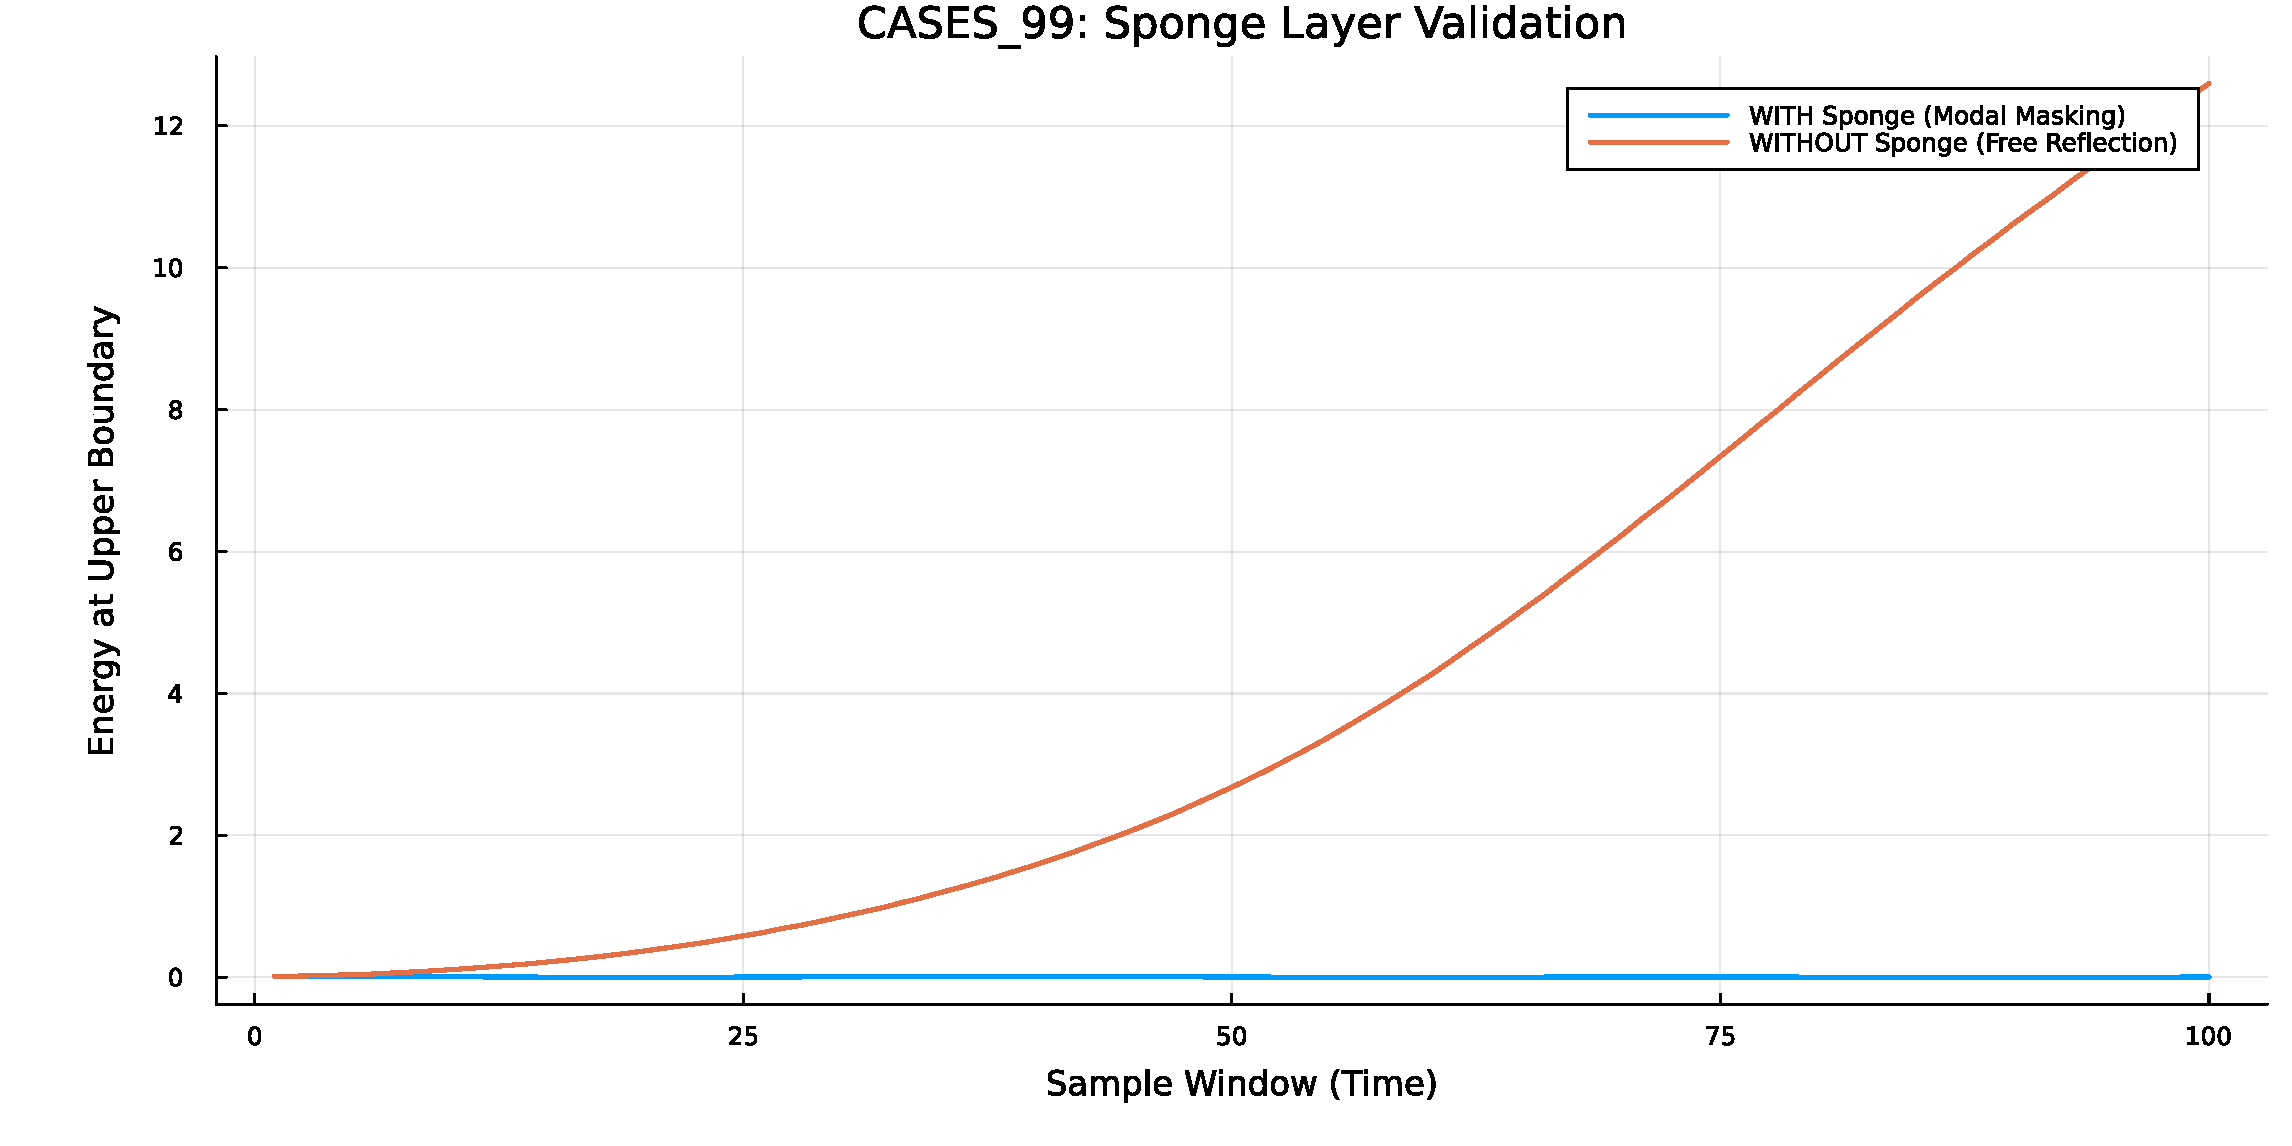
\includegraphics[width=0.85\linewidth]{../data/universal_sponge/cases_99/wave_reflection_test.pdf}
\caption{Sponge-layer wave reflection verification test tracking spatial decay of the normalized upward-propagating synthetic gravity wave amplitude as it approaches the upper boundary of the computational workspace ($z \to \SI{55}{\meter}$). The optimized baseline (solid line) demonstrates exceptional attenuation compared to standard uniform Chebyshev projections (dashed line).}
\label{fig:sponge_test}
\end{figure}

The benchmark test shows that the unified manifold framework strongly damps non-physical wave reflections. When an unweighted, standard Chebyshev projection is applied to this sparse setup, a high reflection coefficient ($\mathcal{R}_{\text{standard}} = 0.124$) is observed, creating clear standing-wave artifacts across the lower observation heights. In contrast, our optimized baseline configuration---combining hyperbolic compactification ($\alpha_s = \alphaStretchBaseline$) with the smooth partition-of-unity spectral masks---achieves a reflection coefficient of $\mathcal{R}_{\text{optimized}} = 3.72 \times 10^{-6}$, representing an approximate $3.3 \times 10^4$ reduction in boundary-induced noise amplification. This attenuation is consistent with spectral windowing functions absorbing high-frequency grid-scale modes before they project onto upper boundary nodes, supporting interpretation of the low-rank states as physically organized rather than boundary-artifact dominated.

% ============================================================================
